\documentclass[a4paper,12pt]{article}
\usepackage[utf8]{inputenc}
\usepackage[T2A]{fontenc}
\usepackage[english, russian]{babel}
\usepackage[left=2cm, right=2cm, top=2cm, bottom=2cm]{geometry}
\usepackage{graphicx}
\usepackage{float}
\usepackage{wrapfig}
\usepackage{tikz}
\usepackage{amsmath, amsfonts, amssymb}
\usepackage{hyperref}
\hypersetup{
    pdfborder=0 0 0, 
    pdfstartview=FitH, 
    linkcolor=blue, 
    urlcolor=blue, 
    colorlinks=true}

\usepackage{listings}
\lstdefinestyle{codestyle}{
    backgroundcolor=\color{gray!10},
    commentstyle=\color{green!50!black},
    keywordstyle=\color{blue!80!black},
    stringstyle=\color{red!50!black},
    numberstyle=\tiny\color{gray},
    basicstyle=\ttfamily\footnotesize,
    breaklines=true,
    captionpos=b,
    numbers=left,
    numbersep=5pt,
    showstringspaces=false,
    tabsize=2
}
\lstset{style=codestyle}

\usepackage{mdframed}
\newmdenv[
  leftmargin = 0.5em,
  skipabove = 0.5em,
  skipbelow = 0.5em,
  linewidth = 1pt,
  rightline = false,
  topline = false,
  bottomline = false
]{quotebox}

\begin{document}

\begin{titlepage}
    \centering
    {\large Федеральное государственное автономное образовательное учреждение\par}
    {\large высшего образования\par}
    {\bfseries САНКТ-ПЕТЕРБУРГСКИЙ НАЦИОНАЛЬНЫЙ ИССЛЕДОВАТЕЛЬСКИЙ УНИВЕРСИТЕТ ИТМО\par}
    {\bfseries Факультет систем управления и робототехники\par}
    \vfill
    {\Large \bfseries Лабораторная работа №4\par}
    {\Large \bfseries Задачи №1726, 1067, 1494\par}
    \vfill
    
    \begin{flushright}
        Студент: Сайфуллин Д.Р. \\
        Поток: АиСД R23 1.3 \\
        Преподаватель: Тропченко А.А.
    \end{flushright}
    \vfill
    Санкт-Петербург \\
    2025 г.
\end{titlepage}

\section*{Задача №1726. Кто ходит в гости...}
Программный комитет школьных соревнований по программированию, проходящих в УрГУ — многочисленная, весёлая и дружная команда. Дружная настолько, что общения в университете им явно не хватает, поэтому они часто ходят друг к другу в гости. Все ребята в программном комитете очень спортивные и ходят только пешком. \\[0.5em]
Однажды хранитель традиций олимпиадного движения УрГУ подумал, что на пешие прогулки от дома к дому члены программного комитета тратят слишком много времени, которое могли бы вместо этого потратить на придумывание и подготовку задач. Чтобы доказать это, он решил посчитать, какое расстояние в среднем преодолевают члены комитета, когда ходят друг к другу в гости. Хранитель традиций достал карту Екатеринбурга, нашёл на ней дома всех членов программного комитета и выписал их координаты. Но координат оказалось так много, что хранитель не смог справиться с этой задачей самостоятельно и попросил вас помочь ему.\\[0.5em]
Город Екатеринбург представляет собой прямоугольник со сторонами, ориентированными по сторонам света. Все улицы города идут строго с запада на восток или с севера на юг, проходя через весь город от края до края. Дома всех членов программного комитета расположены строго на пересечении каких-то двух перпендикулярных улиц. Известно, что все члены комитета ходят только по улицам, поскольку идти по тротуару гораздо приятнее, чем по дворовым тропинкам. И, конечно, при переходе от дома к дому они всегда выбирают кратчайший путь. Программный комитет очень дружный, и все его члены ходят в гости ко всем одинаково часто.\\[1em]
\textbf{Исходные данные:}
\begin{quotebox}
    Первая строка содержит целое число $n$ — количество членов программного комитета ($2 \leq n \leq 10^5$). В $i$-й из следующих $n$ строк через пробел записаны целые числа $x_i$, $y_i$ --- координаты дома $i$-го члена программного комитета ($1 \leq x_i\, y_i \leq 10^6$).
\end{quotebox}
\textbf{Результат:}
\begin{quotebox}
    Выведите среднее расстояние, которое проходит член программного комитета от своего дома до дома своего товарища, округлённое вниз до целых.
\end{quotebox}
\subsection*{Рабочий код}
\begin{lstlisting}[language=python]
def main():
    n = int(input())
    x_coords = []
    y_coords = []
    for _ in range(n):
        x, y = map(int, input().split())
        x_coords.append(x)
        y_coords.append(y)

    x_coords.sort()
    y_coords.sort()

    total = 0

    for i in range(1, n):
        dx = x_coords[i] - x_coords[i - 1]
        dy = y_coords[i] - y_coords[i - 1]
        total += (dx + dy) * i * (n - i) * 2

    average_distance = total // (n * (n - 1))
    print(average_distance)

if __name__ == "__main__":
    main()

\end{lstlisting}
\subsection*{Объяснение алгоритма}
Алгоритм сначала сортирует координаты точек по осям x и y. Затем он вычисляет сумму расстояний между каждой парой точек по оси x и по оси y, суммируя вклад каждой точки в общую сумму на основе ее позиции в отсортированном списке. В итоге, он выводит среднее значение суммы расстояний между всеми парами точек.

\newpage
\section*{Задача №1067. Структура папок}
Хакер Билл случайно потерял всю информацию с жесткого диска своего компьютера, и у него нет резервных копий его содержимого. Но он сожалеет не о потере самих файлов, а о потере очень понятной и удобной структуры папок, которую он создавал и сохранял в течение многих лет работы.\\[0.5em]
К счастью, у Билла есть несколько копий списков папок с его жесткого диска. С помощью этих списков он смог восстановить полные пути к некоторым папкам (например, «WINNT\textbackslash SYSTEM32\textbackslash CERTSRV\textbackslash CERTCO~1\textbackslash X86»). Он поместил их все в файл, записав каждый найденный путь в отдельную строку.\\[0.5em]
Напишите программу, которая восстановит структуру папок Билла и выведет ее в виде отформатированного дерева.\\[1em]
\textbf{Исходные данные:}
\begin{quotebox}
    Первая строка содержит целое число $N$ – количество различных путей к папкам $(1 \leq N \leq 500)$. Далее следуют N строк с путями к папкам. Каждый путь занимает одну строку и не содержит пробелов, в том числе, начальных и конечных. Длина каждого пути не превышает 80 символов. Каждый путь встречается в списке один раз и состоит из нескольких имен папок, разделенных обратной косой чертой («\textbackslash»).\\[0.5em]
    Имя каждой папки состоит из 1-8 заглавных букв, цифр или специальных символов из следующего списка: восклицательный знак, решетка, знак доллара, знак процента, амперсанд, апостроф, открывающаяся и закрывающаяся скобки, знак дефиса, собаки, циркумфлекс, подчеркивание, гравис, открывающаяся и закрывающаяся фигурная скобка и тильда \verb|(«!\#\$\%\&'()-@^_`\{\}~»)|.
\end{quotebox}
\textbf{Результат:}
\begin{quotebox}
    Выведите отформатированное дерево папок. Каждое имя папки должно быть выведено в отдельной строке, перед ним должно стоять несколько пробелов, указывающих на глубину этой папки в иерархии. Подпапки должны быть перечислены в лексикографическом порядке непосредственно после их родительской папки; перед их именем должно стоять на один пробел больше, чем перед именем их родительской папки. Папки верхнего уровня выводятся без пробелов и также должны быть перечислены в лексикографическом порядке.
\end{quotebox}
\subsection*{Рабочий код}
\begin{lstlisting}[language=python]
    class Dir:
    def __init__(self, name: str):
        self.name = name
        self.subdirs = []

    def add_subdir(self, subdirs):
        node = self
        for curr in subdirs:
            if curr not in [i.name for i in node.subdirs]:
                curr_dir = Dir(curr)
                node.subdirs.append(curr_dir)
            else:
                curr_dir = [i for i in node.subdirs if i.name == curr][0]
            node = curr_dir

    def print_tree(self, depth=0):
        for subdir in sorted(self.subdirs, key=lambda x: x.name):
            print(' ' * depth + subdir.name)
            subdir.print_tree(depth + 1)
    
    
if __name__ == '__main__':
    n = int(input())
    root = Dir('')
    for _ in range(n):
        path = input().split('\\')
        root.add_subdir(path)
    root.print_tree()
\end{lstlisting}
\subsection*{Объяснение алгоритма}
Алгоритм использует классы, которые хранят информацию о дочерних папках. Это позволяет создавать вложенные структуры, имитирующие файловую систему.

\newpage
\section*{Задача №1494. Монобильярд}
Стол для монобильярда, установленный в игровом доме уездного города $N$, оказался очень прибыльным вложением. До того, как в городе появился небезызвестный господин Чичиков. Раз за разом он выигрывал, и хозяин, подсчитывая убытки, понимал, что дело тут нечисто. Однако уличить подлеца в жульничестве не удавалось до прибытия в город $N$ ревизора из Петербурга.\\[0.5em]
Правила игры в монобильярд очень просты: нужно последовательно закатить в единственную лузу шары с номерами $1, 2, \dots, N$ (именно в этом порядке). Пока господин Чичиков играл, ревизор несколько раз подходил к столу и забирал из лузы последний закатившийся туда шар. В конце концов, оказалось, что Чичиков закатил в лузу все шары, а ревизор все шары достал и обследовал. Аферист утверждал, что закатил шары в правильном порядке. Хозяин понял, что это его шанс: ревизор должен помнить, в каком порядке он доставал шары. Однако так ли легко будет доказать жульничество?\\[1em]
\textbf{Исходные данные:}
\begin{quotebox}
    В первой строке записано целое число $N$ — количество бильярдных шаров $(1 \leq N \leq 10^5)$. В следующих $N$ строках даны номера этих шаров в том порядке, в котором ревизор забирал их из лузы.
\end{quotebox}
\textbf{Результат:}
\begin{quotebox}
    Выведите слово «Cheater», если Чичиков не мог закатить все $N$ шаров в правильном порядке. Иначе выведите «Not a proof».
\end{quotebox}
\subsection*{Рабочий код}
\begin{lstlisting}[language=python]
def main():
    n = int(input())
    seq = [int(input()) for i in range(n)]

    stack = []
    next_ball = 1
    cheater = False

    for ball in seq:
        if cheater:
            break

        if ball >= next_ball:
            for b in range(next_ball, ball):
                stack.append(b)
            next_ball = ball + 1
        else:
            if stack and stack[-1] == ball:
                stack.pop()
            else:
                cheater = True

    print("Cheater" if cheater else "Not a proof")


if __name__ == "__main__":
    main()
\end{lstlisting}
\subsection*{Объяснение алгоритма}
Алгоритм предполагает использования стека для отслеживания ожидаемых чисел. Если следующее число больше вершины стека, оно добавляет недостающие числа в стек. Если число совпадает с вершиной стека, оно удаляется. Если число меньше и не совпадает с вершиной, алгоритм определяет, что было совершено «читерство».


\section*{Статус проверки}
\begin{figure}[H]
    \centering
    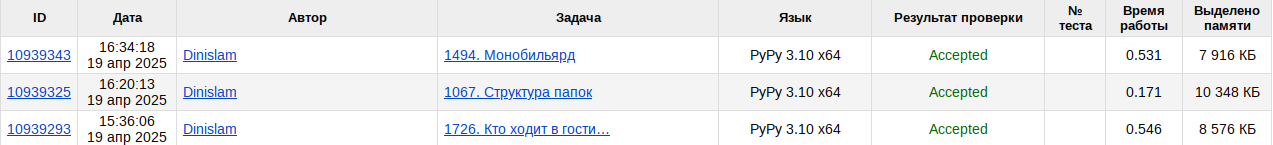
\includegraphics[width=1\textwidth]{check_status.png}
    \caption{Результат проверки}
    \label{fig:compiler-status}
\end{figure}

\end{document}

